% Created by tikzDevice version 0.10.1 on 2018-01-23 02:20:00
% !TEX encoding = UTF-8 Unicode
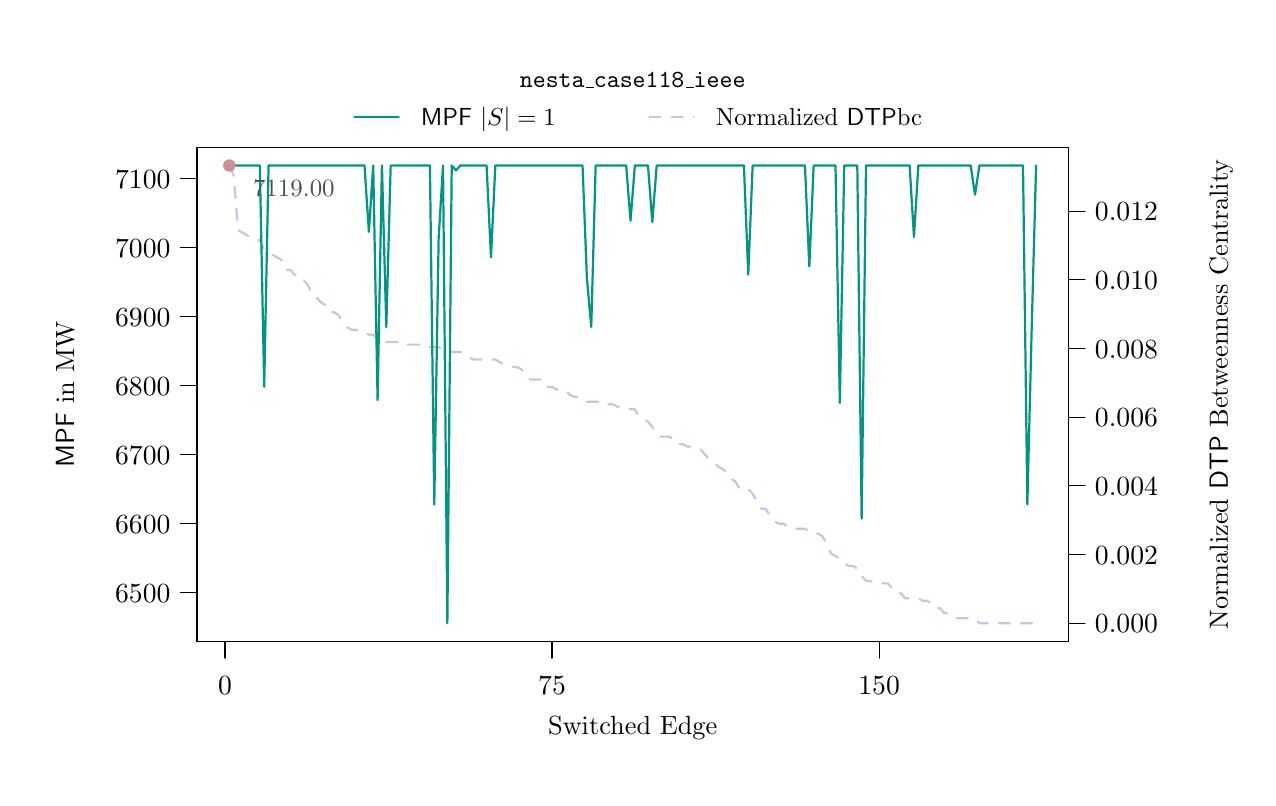
\begin{tikzpicture}[x=1pt,y=1pt]
\definecolor{fillColor}{RGB}{255,255,255}
\path[use as bounding box,fill=fillColor,fill opacity=0.00] (0,0) rectangle (440.85,271.01);
\begin{scope}
\path[clip] (  0.00,  0.00) rectangle (440.85,271.01);
\definecolor{drawColor}{RGB}{193,202,220}

\path[draw=drawColor,line width= 0.8pt,dash pattern=on 4pt off 4pt ,line join=round,line cap=round] ( 72.86,221.20) --
	( 74.44,217.60) --
	( 76.01,197.83) --
	( 77.59,196.93) --
	( 79.16,196.03) --
	( 80.74,195.13) --
	( 82.32,194.23) --
	( 83.89,194.23) --
	( 85.47,190.64) --
	( 87.04,189.74) --
	( 88.62,188.84) --
	( 90.19,187.94) --
	( 91.77,187.04) --
	( 93.35,183.45) --
	( 94.92,183.45) --
	( 96.50,181.65) --
	( 98.07,181.65) --
	( 99.65,179.85) --
	(101.23,178.05) --
	(102.80,174.46) --
	(104.38,173.56) --
	(105.95,171.76) --
	(107.53,170.86) --
	(109.10,168.17) --
	(110.68,168.17) --
	(112.26,167.27) --
	(113.83,164.57) --
	(115.41,162.77) --
	(116.98,161.88) --
	(118.56,161.88) --
	(120.14,160.98) --
	(121.71,160.98) --
	(123.29,160.08) --
	(124.86,160.08) --
	(126.44,158.28) --
	(128.01,157.38) --
	(129.59,157.38) --
	(131.17,157.38) --
	(132.74,157.38) --
	(134.32,157.38) --
	(135.89,156.48) --
	(137.47,156.48) --
	(139.05,156.48) --
	(140.62,156.48) --
	(142.20,156.48) --
	(143.77,156.48) --
	(145.35,155.58) --
	(146.92,155.58) --
	(148.50,155.58) --
	(150.08,154.69) --
	(151.65,153.79) --
	(153.23,153.79) --
	(154.80,153.79) --
	(156.38,153.79) --
	(157.95,152.89) --
	(159.53,151.99) --
	(161.11,151.09) --
	(162.68,151.09) --
	(164.26,151.09) --
	(165.83,151.09) --
	(167.41,151.09) --
	(168.99,151.09) --
	(170.56,150.19) --
	(172.14,149.29) --
	(173.71,148.39) --
	(175.29,148.39) --
	(176.86,148.39) --
	(178.44,147.49) --
	(180.02,145.70) --
	(181.59,143.90) --
	(183.17,143.90) --
	(184.74,143.90) --
	(186.32,143.90) --
	(187.90,141.20) --
	(189.47,141.20) --
	(191.05,140.30) --
	(192.62,140.30) --
	(194.20,140.30) --
	(195.77,138.51) --
	(197.35,137.61) --
	(198.93,137.61) --
	(200.50,136.71) --
	(202.08,135.81) --
	(203.65,135.81) --
	(205.23,135.81) --
	(206.80,135.81) --
	(208.38,134.91) --
	(209.96,134.91) --
	(211.53,134.91) --
	(213.11,134.01) --
	(214.68,134.01) --
	(216.26,134.01) --
	(217.84,133.11) --
	(219.41,133.11) --
	(220.99,130.42) --
	(222.56,129.52) --
	(224.14,128.62) --
	(225.71,126.82) --
	(227.29,124.13) --
	(228.87,123.23) --
	(230.44,123.23) --
	(232.02,123.23) --
	(233.59,121.43) --
	(235.17,120.53) --
	(236.75,120.53) --
	(238.32,119.63) --
	(239.90,119.63) --
	(241.47,119.63) --
	(243.05,118.73) --
	(244.62,116.93) --
	(246.20,115.14) --
	(247.78,114.24) --
	(249.35,112.44) --
	(250.93,111.54) --
	(252.50,110.64) --
	(254.08,107.95) --
	(255.66,107.05) --
	(257.23,104.35) --
	(258.81,104.35) --
	(260.38,104.35) --
	(261.96,102.55) --
	(263.53, 99.86) --
	(265.11, 97.16) --
	(266.69, 97.16) --
	(268.26, 94.46) --
	(269.84, 92.67) --
	(271.41, 91.77) --
	(272.99, 91.77) --
	(274.56, 90.87) --
	(276.14, 90.87) --
	(277.72, 89.97) --
	(279.29, 89.97) --
	(280.87, 89.97) --
	(282.44, 89.07) --
	(284.02, 88.17) --
	(285.60, 88.17) --
	(287.17, 87.27) --
	(288.75, 84.58) --
	(290.32, 80.98) --
	(291.90, 80.08) --
	(293.47, 79.18) --
	(295.05, 77.39) --
	(296.63, 76.49) --
	(298.20, 76.49) --
	(299.78, 75.59) --
	(301.35, 72.89) --
	(302.93, 71.10) --
	(304.51, 71.10) --
	(306.08, 70.20) --
	(307.66, 70.20) --
	(309.23, 70.20) --
	(310.81, 70.20) --
	(312.38, 68.40) --
	(313.96, 66.60) --
	(315.54, 66.60) --
	(317.11, 64.80) --
	(318.69, 64.80) --
	(320.26, 64.80) --
	(321.84, 64.80) --
	(323.41, 63.90) --
	(324.99, 63.90) --
	(326.57, 63.01) --
	(328.14, 61.21) --
	(329.72, 61.21) --
	(331.29, 59.41) --
	(332.87, 59.41) --
	(334.45, 58.51) --
	(336.02, 57.61) --
	(337.60, 57.61) --
	(339.17, 57.61) --
	(340.75, 57.61) --
	(342.32, 57.61) --
	(343.90, 55.82) --
	(345.48, 55.82) --
	(347.05, 55.82) --
	(348.63, 55.82) --
	(350.20, 55.82) --
	(351.78, 55.82) --
	(353.36, 55.82) --
	(354.93, 55.82) --
	(356.51, 55.82) --
	(358.08, 55.82) --
	(359.66, 55.82) --
	(361.23, 55.82) --
	(362.81, 55.82) --
	(364.39, 55.82);
\end{scope}
\begin{scope}
\path[clip] (  0.00,  0.00) rectangle (440.85,271.01);
\definecolor{drawColor}{RGB}{0,0,0}

\path[draw=drawColor,line width= 0.4pt,line join=round,line cap=round] ( 61.20, 49.20) --
	(376.05, 49.20) --
	(376.05,227.81) --
	( 61.20,227.81) --
	( 61.20, 49.20);
\end{scope}
\begin{scope}
\path[clip] (  0.00,  0.00) rectangle (440.85,271.01);
\definecolor{drawColor}{RGB}{0,0,0}

\path[draw=drawColor,line width= 0.4pt,line join=round,line cap=round] (376.05, 55.82) -- (376.05,204.72);

\path[draw=drawColor,line width= 0.4pt,line join=round,line cap=round] (376.05, 55.82) -- (382.05, 55.82);

\path[draw=drawColor,line width= 0.4pt,line join=round,line cap=round] (376.05, 80.63) -- (382.05, 80.63);

\path[draw=drawColor,line width= 0.4pt,line join=round,line cap=round] (376.05,105.45) -- (382.05,105.45);

\path[draw=drawColor,line width= 0.4pt,line join=round,line cap=round] (376.05,130.27) -- (382.05,130.27);

\path[draw=drawColor,line width= 0.4pt,line join=round,line cap=round] (376.05,155.09) -- (382.05,155.09);

\path[draw=drawColor,line width= 0.4pt,line join=round,line cap=round] (376.05,179.91) -- (382.05,179.91);

\path[draw=drawColor,line width= 0.4pt,line join=round,line cap=round] (376.05,204.72) -- (382.05,204.72);

\node[text=drawColor,anchor=base west,inner sep=0pt, outer sep=0pt, scale=  1.00] at (385.65, 52.37) {0.000};

\node[text=drawColor,anchor=base west,inner sep=0pt, outer sep=0pt, scale=  1.00] at (385.65, 77.19) {0.002};

\node[text=drawColor,anchor=base west,inner sep=0pt, outer sep=0pt, scale=  1.00] at (385.65,102.01) {0.004};

\node[text=drawColor,anchor=base west,inner sep=0pt, outer sep=0pt, scale=  1.00] at (385.65,126.83) {0.006};

\node[text=drawColor,anchor=base west,inner sep=0pt, outer sep=0pt, scale=  1.00] at (385.65,151.64) {0.008};

\node[text=drawColor,anchor=base west,inner sep=0pt, outer sep=0pt, scale=  1.00] at (385.65,176.46) {0.010};

\node[text=drawColor,anchor=base west,inner sep=0pt, outer sep=0pt, scale=  1.00] at (385.65,201.28) {0.012};
\end{scope}
\begin{scope}
\path[clip] (  0.00,  0.00) rectangle (440.85,271.01);
\definecolor{drawColor}{RGB}{0,150,130}

\path[draw=drawColor,line width= 0.8pt,line join=round,line cap=round] ( 72.86,221.20) --
	( 74.44,221.20) --
	( 76.01,221.20) --
	( 77.59,221.20) --
	( 79.16,221.20) --
	( 80.74,221.20) --
	( 82.32,221.20) --
	( 83.89,221.20) --
	( 85.47,141.26) --
	( 87.04,221.20) --
	( 88.62,221.20) --
	( 90.19,221.20) --
	( 91.77,221.20) --
	( 93.35,221.20) --
	( 94.92,221.20) --
	( 96.50,221.20) --
	( 98.07,221.20) --
	( 99.65,221.20) --
	(101.23,221.20) --
	(102.80,221.20) --
	(104.38,221.20) --
	(105.95,221.20) --
	(107.53,221.20) --
	(109.10,221.20) --
	(110.68,221.20) --
	(112.26,221.20) --
	(113.83,221.20) --
	(115.41,221.20) --
	(116.98,221.20) --
	(118.56,221.20) --
	(120.14,221.20) --
	(121.71,221.20) --
	(123.29,197.25) --
	(124.86,221.20) --
	(126.44,136.39) --
	(128.01,221.20) --
	(129.59,162.79) --
	(131.17,221.20) --
	(132.74,221.20) --
	(134.32,221.20) --
	(135.89,221.20) --
	(137.47,221.20) --
	(139.05,221.20) --
	(140.62,221.20) --
	(142.20,221.20) --
	(143.77,221.20) --
	(145.35,221.20) --
	(146.92, 98.72) --
	(148.50,194.73) --
	(150.08,221.20) --
	(151.65, 55.82) --
	(153.23,221.20) --
	(154.80,219.45) --
	(156.38,221.20) --
	(157.95,221.20) --
	(159.53,221.20) --
	(161.11,221.20) --
	(162.68,221.20) --
	(164.26,221.20) --
	(165.83,221.20) --
	(167.41,188.02) --
	(168.99,221.20) --
	(170.56,221.20) --
	(172.14,221.20) --
	(173.71,221.20) --
	(175.29,221.20) --
	(176.86,221.20) --
	(178.44,221.20) --
	(180.02,221.20) --
	(181.59,221.20) --
	(183.17,221.20) --
	(184.74,221.20) --
	(186.32,221.20) --
	(187.90,221.20) --
	(189.47,221.20) --
	(191.05,221.20) --
	(192.62,221.20) --
	(194.20,221.20) --
	(195.77,221.20) --
	(197.35,221.20) --
	(198.93,221.20) --
	(200.50,221.20) --
	(202.08,180.36) --
	(203.65,162.84) --
	(205.23,221.20) --
	(206.80,221.20) --
	(208.38,221.20) --
	(209.96,221.20) --
	(211.53,221.20) --
	(213.11,221.20) --
	(214.68,221.20) --
	(216.26,221.20) --
	(217.84,201.27) --
	(219.41,221.20) --
	(220.99,221.20) --
	(222.56,221.20) --
	(224.14,221.20) --
	(225.71,200.75) --
	(227.29,221.20) --
	(228.87,221.20) --
	(230.44,221.20) --
	(232.02,221.20) --
	(233.59,221.20) --
	(235.17,221.20) --
	(236.75,221.20) --
	(238.32,221.20) --
	(239.90,221.20) --
	(241.47,221.20) --
	(243.05,221.20) --
	(244.62,221.20) --
	(246.20,221.20) --
	(247.78,221.20) --
	(249.35,221.20) --
	(250.93,221.20) --
	(252.50,221.20) --
	(254.08,221.20) --
	(255.66,221.20) --
	(257.23,221.20) --
	(258.81,221.20) --
	(260.38,181.82) --
	(261.96,221.20) --
	(263.53,221.20) --
	(265.11,221.20) --
	(266.69,221.20) --
	(268.26,221.20) --
	(269.84,221.20) --
	(271.41,221.20) --
	(272.99,221.20) --
	(274.56,221.20) --
	(276.14,221.20) --
	(277.72,221.20) --
	(279.29,221.20) --
	(280.87,221.20) --
	(282.44,184.78) --
	(284.02,221.20) --
	(285.60,221.20) --
	(287.17,221.20) --
	(288.75,221.20) --
	(290.32,221.20) --
	(291.90,221.20) --
	(293.47,135.43) --
	(295.05,221.20) --
	(296.63,221.20) --
	(298.20,221.20) --
	(299.78,221.20) --
	(301.35, 93.62) --
	(302.93,221.20) --
	(304.51,221.20) --
	(306.08,221.20) --
	(307.66,221.20) --
	(309.23,221.20) --
	(310.81,221.20) --
	(312.38,221.20) --
	(313.96,221.20) --
	(315.54,221.20) --
	(317.11,221.20) --
	(318.69,221.20) --
	(320.26,195.34) --
	(321.84,221.20) --
	(323.41,221.20) --
	(324.99,221.20) --
	(326.57,221.20) --
	(328.14,221.20) --
	(329.72,221.20) --
	(331.29,221.20) --
	(332.87,221.20) --
	(334.45,221.20) --
	(336.02,221.20) --
	(337.60,221.20) --
	(339.17,221.20) --
	(340.75,221.20) --
	(342.32,210.67) --
	(343.90,221.20) --
	(345.48,221.20) --
	(347.05,221.20) --
	(348.63,221.20) --
	(350.20,221.20) --
	(351.78,221.20) --
	(353.36,221.20) --
	(354.93,221.20) --
	(356.51,221.20) --
	(358.08,221.20) --
	(359.66,221.20) --
	(361.23, 98.72) --
	(362.81,162.84) --
	(364.39,221.20);
\end{scope}
\begin{scope}
\path[clip] (  0.00,  0.00) rectangle (440.85,271.01);
\definecolor{drawColor}{RGB}{0,0,0}

\path[draw=drawColor,line width= 0.4pt,line join=round,line cap=round] ( 61.20, 49.20) --
	(376.05, 49.20) --
	(376.05,227.81) --
	( 61.20,227.81) --
	( 61.20, 49.20);
\end{scope}
\begin{scope}
\path[clip] (  0.00,  0.00) rectangle (440.85,271.01);
\definecolor{drawColor}{RGB}{0,0,0}

\path[draw=drawColor,line width= 0.4pt,line join=round,line cap=round] ( 61.20, 66.79) -- ( 61.20,216.46);

\path[draw=drawColor,line width= 0.4pt,line join=round,line cap=round] ( 61.20, 66.79) -- ( 55.20, 66.79);

\path[draw=drawColor,line width= 0.4pt,line join=round,line cap=round] ( 61.20, 91.74) -- ( 55.20, 91.74);

\path[draw=drawColor,line width= 0.4pt,line join=round,line cap=round] ( 61.20,116.68) -- ( 55.20,116.68);

\path[draw=drawColor,line width= 0.4pt,line join=round,line cap=round] ( 61.20,141.62) -- ( 55.20,141.62);

\path[draw=drawColor,line width= 0.4pt,line join=round,line cap=round] ( 61.20,166.57) -- ( 55.20,166.57);

\path[draw=drawColor,line width= 0.4pt,line join=round,line cap=round] ( 61.20,191.51) -- ( 55.20,191.51);

\path[draw=drawColor,line width= 0.4pt,line join=round,line cap=round] ( 61.20,216.46) -- ( 55.20,216.46);

\node[text=drawColor,anchor=base east,inner sep=0pt, outer sep=0pt, scale=  1.00] at ( 51.60, 63.35) {6500};

\node[text=drawColor,anchor=base east,inner sep=0pt, outer sep=0pt, scale=  1.00] at ( 51.60, 88.29) {6600};

\node[text=drawColor,anchor=base east,inner sep=0pt, outer sep=0pt, scale=  1.00] at ( 51.60,113.24) {6700};

\node[text=drawColor,anchor=base east,inner sep=0pt, outer sep=0pt, scale=  1.00] at ( 51.60,138.18) {6800};

\node[text=drawColor,anchor=base east,inner sep=0pt, outer sep=0pt, scale=  1.00] at ( 51.60,163.13) {6900};

\node[text=drawColor,anchor=base east,inner sep=0pt, outer sep=0pt, scale=  1.00] at ( 51.60,188.07) {7000};

\node[text=drawColor,anchor=base east,inner sep=0pt, outer sep=0pt, scale=  1.00] at ( 51.60,213.01) {7100};
\end{scope}
\begin{scope}
\path[clip] (  0.00,  0.00) rectangle (440.85,271.01);
\definecolor{fillColor}{RGB}{207,142,147}

\path[fill=fillColor] ( 72.86,221.20) circle (  2.25);
\end{scope}
\begin{scope}
\path[clip] (  0.00,  0.00) rectangle (440.85,271.01);
\definecolor{drawColor}{RGB}{0,0,0}

\path[draw=drawColor,line width= 0.4pt,line join=round,line cap=round] ( 61.20, 49.20) --
	(376.05, 49.20) --
	(376.05,227.81) --
	( 61.20,227.81) --
	( 61.20, 49.20);
\end{scope}
\begin{scope}
\path[clip] (  0.00,  0.00) rectangle (440.85,271.01);
\definecolor{drawColor}{gray}{0.30}

\node[text=drawColor,anchor=base,inner sep=0pt, outer sep=0pt, scale=  0.90] at ( 96.18,210.04) {7119.00};
\end{scope}
\begin{scope}
\path[clip] (  0.00,  0.00) rectangle (440.85,271.01);
\definecolor{drawColor}{RGB}{0,0,0}

\path[draw=drawColor,line width= 0.4pt,line join=round,line cap=round] ( 71.29, 49.20) -- (307.66, 49.20);

\path[draw=drawColor,line width= 0.4pt,line join=round,line cap=round] ( 71.29, 49.20) -- ( 71.29, 43.20);

\path[draw=drawColor,line width= 0.4pt,line join=round,line cap=round] (189.47, 49.20) -- (189.47, 43.20);

\path[draw=drawColor,line width= 0.4pt,line join=round,line cap=round] (307.66, 49.20) -- (307.66, 43.20);

\node[text=drawColor,anchor=base,inner sep=0pt, outer sep=0pt, scale=  1.00] at ( 71.29, 30.00) {0};

\node[text=drawColor,anchor=base,inner sep=0pt, outer sep=0pt, scale=  1.00] at (189.47, 30.00) {75};

\node[text=drawColor,anchor=base,inner sep=0pt, outer sep=0pt, scale=  1.00] at (307.66, 30.00) {150};

\node[text=drawColor,anchor=base,inner sep=0pt, outer sep=0pt, scale=  0.95] at (218.62, 15.60) {Switched Edge};

\node[text=drawColor,rotate= 90.00,anchor=base,inner sep=0pt, outer sep=0pt, scale=  0.95] at ( 16.80,138.51) {$\mathsf{MPF}$ in~$\mathrm{MW}$};

\node[text=drawColor,rotate= 90.00,anchor=base,inner sep=0pt, outer sep=0pt, scale=  0.95] at (433.65,138.51) {Normalized~$\mathsf{DTP}$ Betweenness Centrality};
\end{scope}
\begin{scope}
\path[clip] (  0.00,  0.00) rectangle (440.85,271.01);
\definecolor{drawColor}{RGB}{0,150,130}

\path[draw=drawColor,line width= 0.8pt,line join=round,line cap=round] (118.04,238.60) -- (134.06,238.60);
\definecolor{drawColor}{RGB}{193,202,220}

\path[draw=drawColor,line width= 0.8pt,dash pattern=on 4pt off 4pt ,line join=round,line cap=round] (224.63,238.60) -- (240.65,238.60);
\definecolor{drawColor}{RGB}{0,0,0}

\node[text=drawColor,anchor=base,inner sep=0pt, outer sep=0pt, scale=  0.89] at (218.62,249.28) {\texttt{nesta\_case118\_ieee}};

\node[text=drawColor,anchor=base west,inner sep=0pt, outer sep=0pt, scale=  0.89] at (142.07,235.54) {$\mathsf{MPF}~|S|=1$};

\node[text=drawColor,anchor=base west,inner sep=0pt, outer sep=0pt, scale=  0.89] at (248.66,235.54) {Normalized~$\mathsf{DTP}$bc};
\end{scope}
\end{tikzpicture}
